\chapter{Implementation}
\thispagestyle{main} % Needed for Footer and Header on Chapterpage
This chapter focuses on explaining why things were implemented in a certain manner. In this chapter the trade-offs and decisions which were made while building the VM are described in a manner that follow up works get a better understanding of why some parts of the VM are implemented in a certain way so that they either are more certain when changing something or to help them reach the same conclusion faster.

\section{Software architecture}
Figure \ref{package overview} shows the structure of the project on package-level and the dependencies among them. The miner application was built with software engineering principles in mind. Particular attention was paid to modularity. This made it easy to integrate the virtual machine into the existing miner application. Furthermore the following figure shows which packages were added and which where modified to successfully integrate the execution of smart contracts into the Bazo blockchain.
\begin{figure}[H]
	\begin{center}
	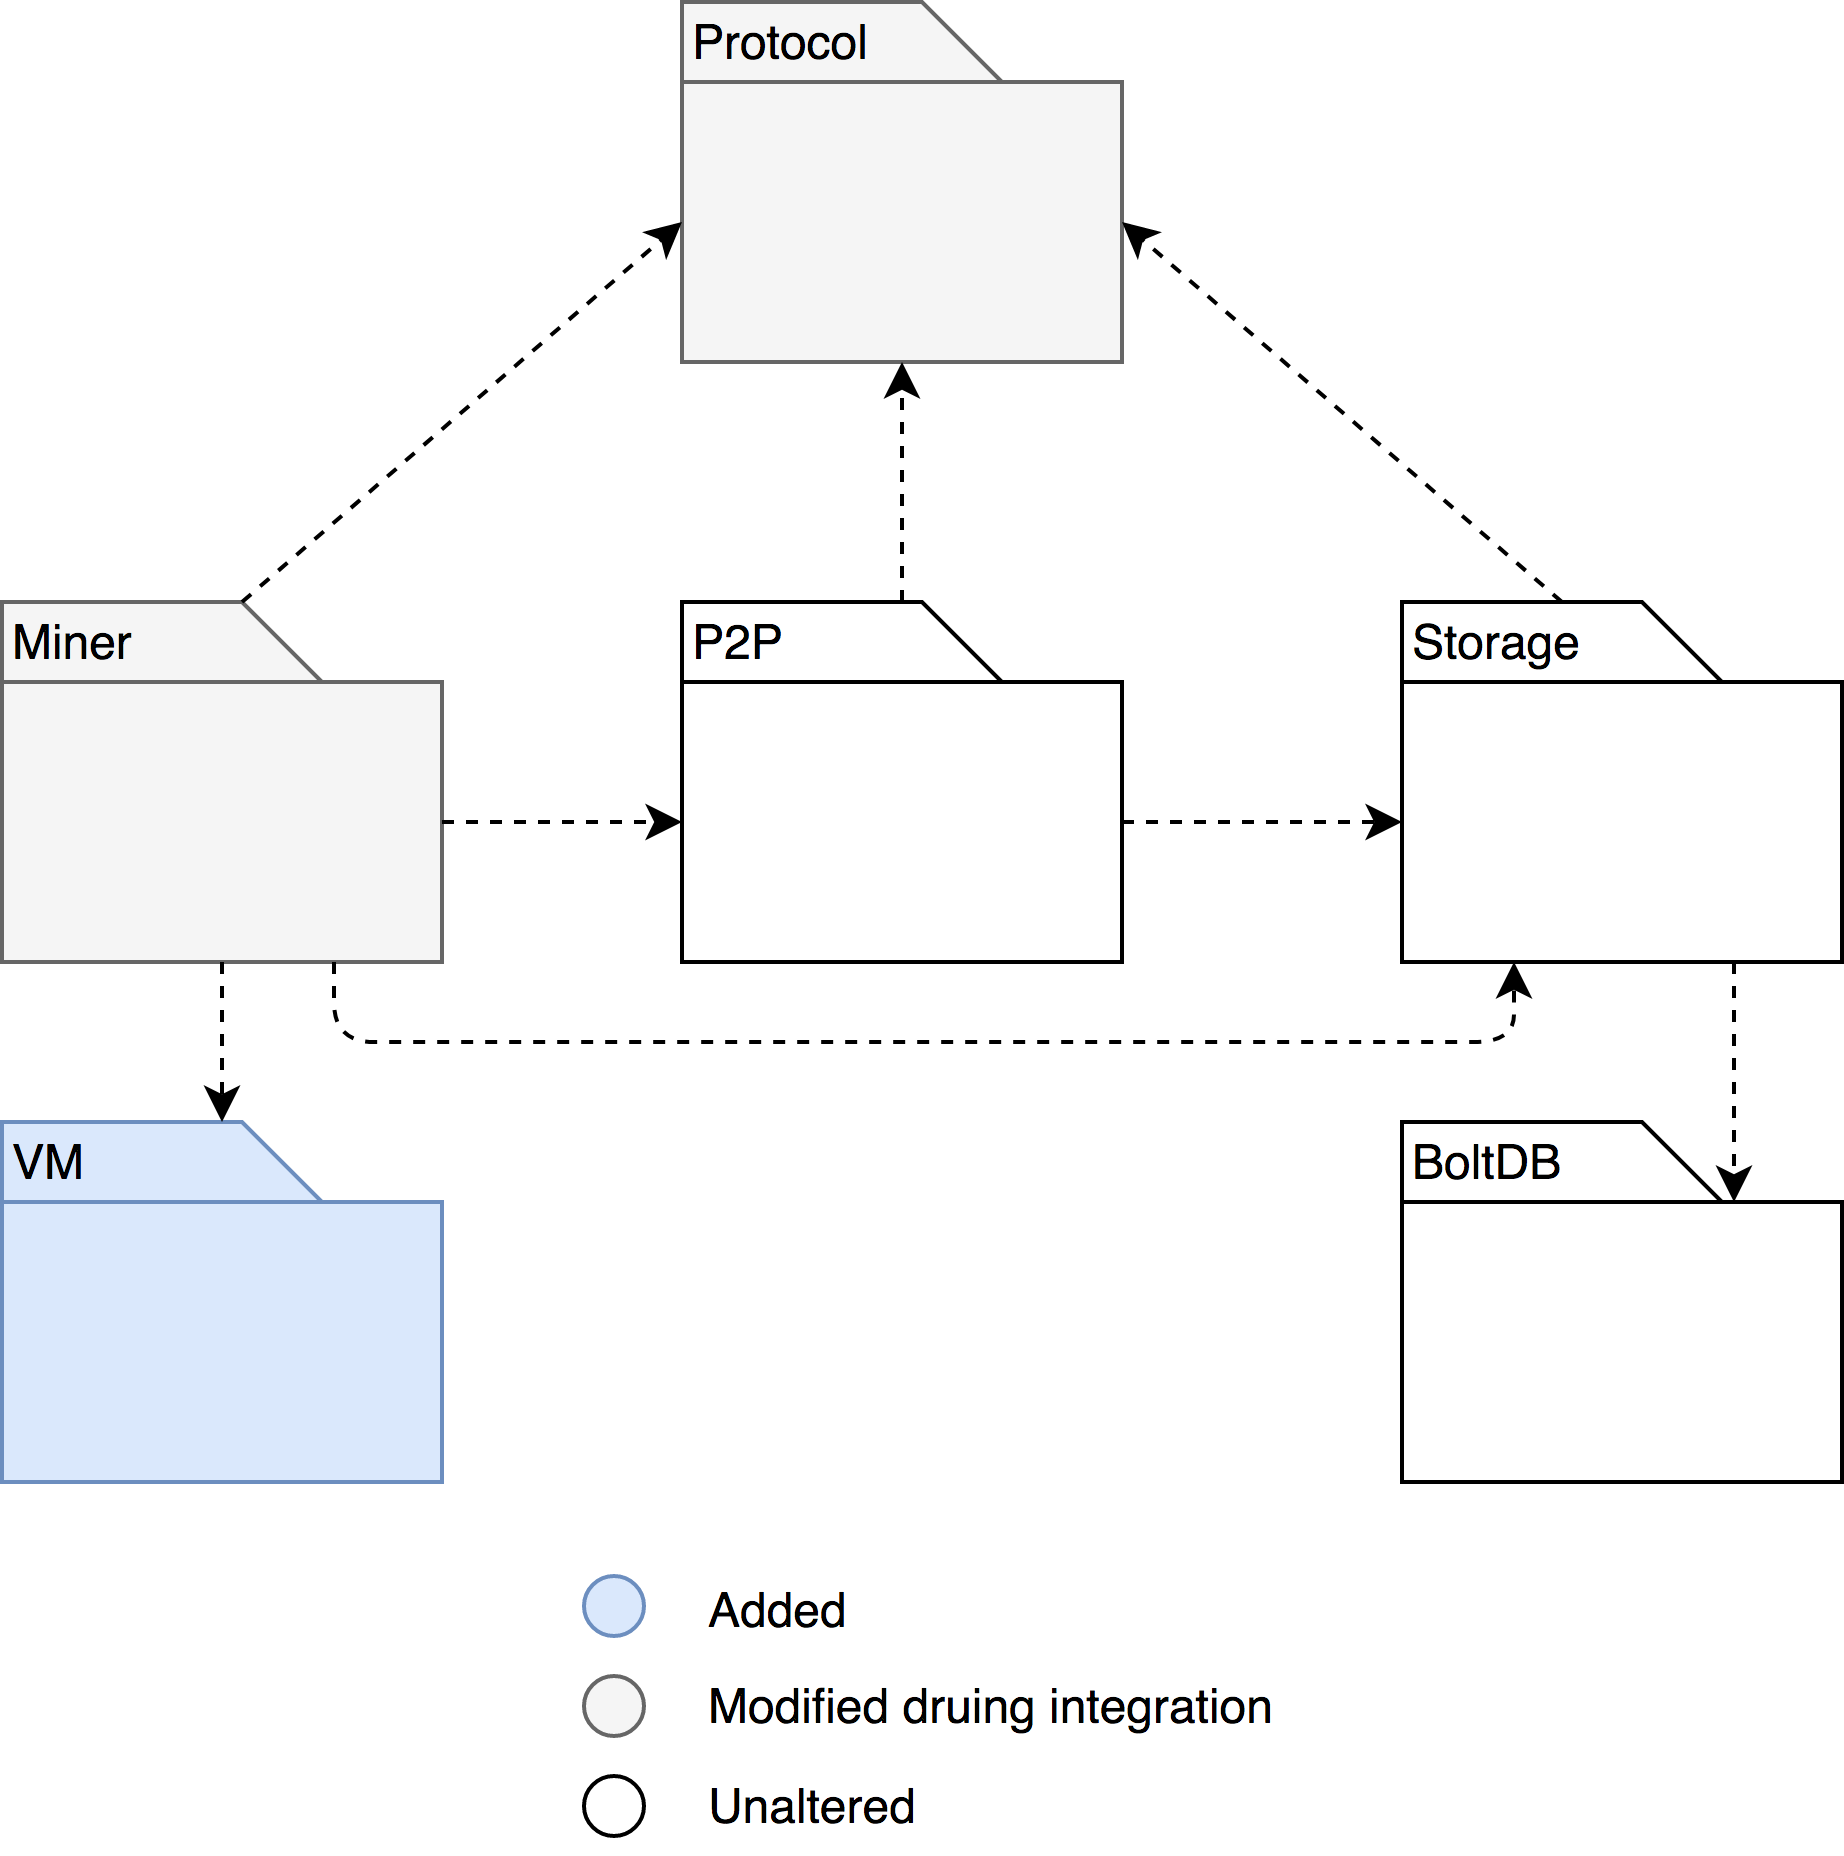
\includegraphics[width=0.9\textwidth]{./images/package-diagram}
	\caption{UML Package Diagram}
	\label{package overview}
	\end{center}
  \end{figure}
  
\begin{description}
	\item[Protocol] This package contains the building blocks for the Bazo blockchain. In particular it contains the structure, encoding, decoding and hashing functions of all transaction types, blocks and accounts. In addition a transaction interface is defined, allowing an abstract treatment of transactions. \cite{ba_miner}
	\item[Miner] The miner package contains all mining related components. That includes the validation and consolidation of transactions into blocks, the calculation of the consensus mechanism and the building of the merkle tree. In addition to that, blockchain related tasks itself such as rollback operation and state changes are contained in this package. Access to P2P and Storage packages are needed in order to handle transactions over the network and signal storage-related operations. \cite{ba_miner} To execute the virtual machine and access its results, the miner also needs access to the VM package.
	\item[VM] This package contains the virtual machine itself and all its components, namely the evaluation stack, the call stack, implementations of data structures that can be used by the virtual machine such as array and map and all available opcodes. 
	\item[P2P] All networking related operations are implemented in the P2P package \cite{ba_miner}. Since for the integration of the virtual machine nothing had to be changed, the content of this package is not discussed any further.
	\item[Storage] The storage package is concerned with memory-related tasks. The lower-level functionality was implemented with the external BoltDB package. Since entries are encoded before writing to storage and decoded when loaded \cite{ba_miner}, this package could be left unaltered. For that reason, this package is also not described further.
	\item[BoltDB] This package shows the BoltDB package which is an external dependency. BoltDB is a simple, lightweight key/value base. \cite{ba_miner}
	\item[Parser] The Parser package contains the parser, which consists of a Tokenize and Parse function and tokens. This components are needed to compile \flqq Enhanced Bazo byte code\frqq{ } to a byte code instruction set that can be interpreted by the virtual machine. This package is completely stand-alone and does not have any dependencies. The package is also kept in a separate repository.
\end{description}

\section{Contract execution}

\section{VM Package overview}
As the miner and all other projects are written in golang, for this project also golang is used.
At the time of writing this thesis the VM consists of the following classes:
% Insert execution cycle graphic

\section{GAS}

\section{Trace Function}

\section{Stack}

% TODO insert crc card for stack

\subsection{Maximum stack size}
Facing the concern of excess memory usage of the contract on the miner, we decided to limit the stack size to 1MB which seems to be well above what the contracts will need. We neglected using the gas amount for max storage determination because it would be just a soft limit

\subsection{Maximum variable size}
Since it is possible to easily craft denial of service attacks for the blockchain if there is no limit on the variable size we decided to set the variable size to a specific fixed amount instead of arbitrary precision.

\subsection{Data structure}
As underlying data structure of "Stack", keeping in mind to keep the code of the vm short and simple, we decided to use an array of big.Int. It was important that the datatype used for the underlying datatype was of arbitrary length because splitting up an element into multiple bytes so that it can be saved when using an array of bytes as underlying data structure would have been a lot more complex and more error-prone. Arbitrary length is implemented for example an array of jagged arrays of bytes. On the vm it was very important that the type used in the vm provided mathematical methods and also that it could store and work with values of up to 256 bit size. Only big.Int fulfilled both requirements and therefore it was choosen for the vm. Thanks to big.Int being of arbitrary length we could then use an array of big.Int as underlying data structure which also simplifies our code since we don't have to cast the values retrieved from the stack before working with them.

We neglected working with pointers because even though there are more elements created on the heap of the physical machine, it shouldn't make a difference considering the vast availability of resources on modern computers and our rather small contracts. We neglected using a simple array of bytes as the whole data structure where different datatypes are read using a different amount of bytes, as it is common when having no abstraction layer or using a jagged array of byte arrays because the could becomes a lot more readable in the vm and less conversions from big.Int to byte array are necessary. We accept the dependency on the datatype big.Int which is necessary as it implements all mathematical operations which are very important and because it is of arbitrary precision and the size of other datatypes would not have been sufficient especially for cryptographic purposes.

\section{Virtual machine}
The virtual machine itself is implemented as a switch case where it takes different bytes and determines what has to be executed on each value.

% TODO insert crc card for vm
\subsection{opCodes}
% Please add the following required packages to your document preamble:
% \usepackage{booktabs}
\begin{table}[]
\centering
\caption{List of opCodes available}
\label{opcodes cheat sheet}
\begin{tabular}{@{}llll@{}}
\toprule
\textbf{Instruction} & \textbf{Mnemonic} & \textbf{opCode} & \textbf{Description}                                     \\ \midrule
Push Bytes           & PUSH              & 0x00            & stack $\leftarrow$ bytes                                            \\
Duplicate            & DUP               & 0x01            & stack $\leftarrow$ peek1                           \\
Roll                 & ROLL              & 0x02            & removes element at index and push to ToS           \\
Pop                  & POP               & 0x03            & pops ToS                                                 \\
Add                  & ADD               & 0x04            & stack $\leftarrow$ pop1 \+ pop2                                      \\
Subtract             & SUB               & 0x05            & stack $\leftarrow$ pop1 \- pop2                                      \\
Multiply             & MULT              & 0x06            & stack $\leftarrow$ pop1 \* pop2                                      \\
Divide               & DIV               & 0x07            & stack $\leftarrow$ pop1 \/ pop2                                      \\
Modulo               & MOD               & 0x08            & stack $\leftarrow$ pop1 \% pop2                                     \\
Negate               & NEG               & 0x09            & stack $\leftarrow$ todo                                             \\
Equals               & EQ                & 0x0a            & stack $\leftarrow$ 1 if pop1 == pop2, 0 otherwise                   \\
Not equal            & NEQ               & 0x0b            & stack $\leftarrow$ 1 if pop1 != pop2, 0 otherwise                   \\
Lower than           & LT                & 0x0c            & stack $\leftarrow$ 1 if pop1 \textless{} pop2, 0 otherwise            \\
Greater than         & GT                & 0x0d            & stack $\leftarrow$ 1 if pop1 \textgreater{} pop2, 0 otherwise         \\
Lower than/equals    & LTE               & 0x0e            & stack $\leftarrow$ 1 if pop1 \textless{}= pop2, 0 otherwise         \\
Greater than/equals  & GTE               & 0x0f            & stack $\leftarrow$ 1 if pop1 \textgreater{}= pop2, 0 otherwise      \\
Shift left           & SHIFTL            & 0x10            & stack $\leftarrow$ pop 1 \textless{}\textless nrOfShifts            \\
Shift right          & SHIFTR            & 0x11            & stack $\leftarrow$ pop 1 \textgreater{}\textgreater nrOfShifts      \\
No operation         & NOP               & 0x12            & does nothing                                             \\
Jump                 & JMP               & 0x13            & jump to address                                          \\
Jump if true         & JMPIF             & 0x14            & jumps to address if pop1 == 1                            \\
Call                 & CALL              & 0x15            & call a function                                          \\
Call if true         & CALLIF            & 0x16            & calls a function if pop1 == 1                            \\
Call external        & CALLEXT           & 0x17            & calls function from external smart contract              \\
Return               & RET               & 0x18            & returns from function                                    \\
Size of ToS          & SIZE              & 0x19            & stack $\leftarrow$ size(pop1)                                       \\
Store                & STORE             & 0x1a            & stores pop1 in callStack                                 \\
State Store          & SSTORE            & 0x1b            & stores pop1 in contractVariables                         \\
Load                 & LOAD              & 0x1c            & stack $\leftarrow$ var from callStack
    \\
State Load           & SLOAD             & 0x1d            & stack $\leftarrow$ receiver var from contractVariables \\
Address              & ADDRESS           & 0x1e            & stack $\leftarrow$ receiver account address                         \\
Balance              & BALANCE           & 0x1f            & stack $\leftarrow$ receiver account balance                         \\
Caller               & CALLER            & 0x20            & stack $\leftarrow$ contract caller                                  \\
Call value           & CALLVAL           & 0x21            & stack $\leftarrow$ transaction amount in bazo coins                 \\
Call data            & CALLDATA          & 0x22            & stack $\leftarrow$ transaction data                                 \\
New map              & NEWMAP            & 0x23            & stack $\leftarrow$ new map                                          \\
Map push             & MAPPUSH           & 0x24            & stack $\leftarrow$ add entry to map                                 \\
Map get value        & MAPGETVAL         & 0x25            & todo                                                     \\
Map set value        & MAPSETVAL         & 0x26            & todo                                                     \\
Map remove           & MAPREMOVE         & 0x27            & todo                                                     \\
New array            & NEWARR            & 0x28            & stack $\leftarrow$ new array                                        \\
Array append         & ARRAPPEND         & 0x29            & todo                                                     \\
Array insert         & ARRINSERT         & 0x2a            & todo                                                     \\
Array remove         & ARRREMOVE         & 0x2b            & todo                                                     \\
Array index at       & ARRAT             & 0x2c            & todo                                                     \\
SHA3 Hashing         & SHA3              & 0x2d            & stack $\leftarrow$ SHA3\_HASH(pop 1)                                \\
Check signature      & CHECKSIG          & 0x2e            & todo                                                     \\
Halt with error      & ERRHALT           & 0x2f            & return from Exec() function with false                   \\
Halt                 & HALT              & 0x30            & return from Exec() function with true                    \\ \bottomrule
\end{tabular}
\end{table}

\subsubsection{call stack}

\subsubsection{Arithmetic}

\subsubsection{Bitoperations}


\subsubsection{Controlflowoperations}


\subsubsection{Datastructures}
The datastructures the vm can create are map, array and struct on top of an array. 




\begin{tabular}[t]{ p{3cm} p{12.5cm}}
\textbf{NEWMAP} & 
The opcode NEWMAP creates a new map and pushes it on the stack. 
\\ \\

\textbf{MAPPUSH} & 
\\ \\

\textbf{MAPGETVAL} & 
\\ \\

\end{tabular}

The two basic datastructures map and array are directly implemented as opcodes



describe the implementation of map, array and how one could create a struct. Do it the same as the other opcodes.

Structs could be implemented using a 



\subsection{Context}

For the vm execution to have any effect it is necessary to change the state of the miner eventually. The problem with an immediate change of the miner state is that the contract execution could fail in the middle of the contract resulting in inconsistencies. Such inconsistencies could be resolved with rollback but since this is rather difficult to implement because something keeping track of the changed data, it was decided to provide the state as a copy in a context object. The VM would later on perform the changes to contract data. The changed contract data would later on be written back by the miner after a successfull contract execution


This was implemented using an interface because all the methods the VM can use are easily readable in the interface 

which made it possible to create a special context mock type for testing and one for the actual miner implementation. This was and is useful when having to redefine methods, it also makes it more clear to what the vm actually has acces via reading the context interface. 


Since the state of the vm is not persisted 

The context describes all variables outside the 

\subsection{Sideffects on data}

Since the VM operates on copies the values will also not be changed by a faulty contract.

\section{Miner integration}

\subsection{Adjustment of Transaction Encoding}

\subsection{Adjustment of opcodes to context and miner}

\subsection{Testing}
\subsubsection{Test Driven Development}
The project was implemented with test driven development. 

\subsubsection{Fuzz Testing}
An instruction in a smart contract must never be able to crash the miner. Calling a smart contract function with malicious instructions would cause the whole blockchain to collapse. To check if the VM fails gracefully, a fuzz test was implemented which creates contracts with real random bytes and then executes them. Contracts causing the miner to crash were reproduced as unit test in order to find the bug. Once the bug was fixed it was mitigated. This process was repeated over and over again. Starting the fuzz test with five million random contracts with every commit to the remote repository and having run it with a billion random contracts over night makes us confident that every bug was found and mitigated.

\subsection{Error handling}
Since the VM just processes one operation code after the other and the smart contracts have to be written directly in these opcodes it is easily possible to write byte code which is not possible for the vm to execute, for example byte code which tells the vm to push six bytes on the stack when there is only one byte left in the instruction set. This of course means that an error occurs somewhere in the vm which could terminate the miner. This should neither be possible by accident nor by choice.

Therefore it was paid a lot of attention to put guards around functions possibly throwing an error to avoid calling accordant functions with invalid values and define graceful failures with an error object. The message of this error object is later on pushed on the stack of the vm after that the vm halts. Also to make the debugging less complicated, the name of the opcode in which the error occoured is added to the front of the error code, therefore it is possible to determine what caused the error up to instruction kind.

%insert number of testcoverage

\section{Contracts}

\subsection{Tokenization Contract}

\subsection{Benchmarking Contract}
The benchmarking contract has been implemented in solidity, as a golang programm directly and with the opcodes of our VM. 

The goal is to compare the overhead
